\begin{frame}[fragile]{Visualização do {\it quicksort}}

    \begin{figure}
        \centering

        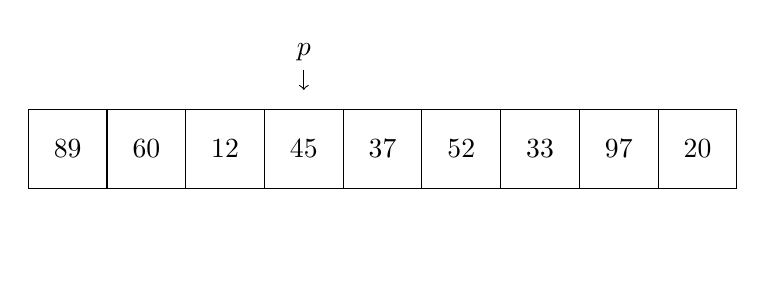
\begin{tikzpicture}
            \draw (0, 5) grid (9, 6);

            \draw[->] (3.5,6.5) node[anchor=south] { $p$ } -- (3.5,6.25);
            \draw[opacity=0,->] (1.5,4.5) node[anchor=north] { $i$ } -- (1.5,4.75);
            \draw[opacity=0,->] (1.5,6.5) node[anchor=south] { $j$ } -- (1.5,6.25);

            \node at (0.5, 5.5) { \textcolor{black}{$89$} };
            \node at (1.5, 5.5) { \textcolor{black}{$60$} };
            \node at (2.5, 5.5) { \textcolor{black}{$12$} };
            \node at (3.5, 5.5) { \textcolor{black}{$45$} };
            \node at (4.5, 5.5) { \textcolor{black}{$37$} };
            \node at (5.5, 5.5) { \textcolor{black}{$52$} };
            \node at (6.5, 5.5) { \textcolor{black}{$33$} };
            \node at (7.5, 5.5) { \textcolor{black}{$97$} };
            \node at (8.5, 5.5) { \textcolor{black}{$20$} };

        \end{tikzpicture}

    \end{figure}

\end{frame}

